\setcounter{page}{1}
\section*{Zielsetzung}
Elektronen in Halbleiternanostrukturen, deren Abmessungen im Nanometerbereich liegen,
erfahren einen räumlichen Einschluss. In kolloidalen Nanokristallen erfolgt dieser Einschluss
in allen drei Raumrichtungen, was zu rein diskreten Energiespektren führt, die von Atomen bekannt sind.
Durch Einstellung der Größe und der chemischen Zusammensetzung lassen sich die opto-elektronischen
Eigenschaften der Kristalle fast beliebig einstellen, was sie aus technischer Sicht extrem interessant macht~\cite{dissArens}.
Die räumliche Begrenzung der Elektronen-Wellenfunktionen führt zu einer ausgeprägten Lumineszenz, die
in diesem Experiment untersucht werden soll.

\section{Theorie}
\label{sec:theo}
Nachfolgend sollen zunächst einige theoretische Überlegungen zu Halbleiter-Nanokristallen vorgestellt werden, die
zum Verständnis der durchgeführten Messungen notwendig sind. Es soll insbesondere motiviert werden, wie die
Photolumineszenzspektren mit der Zusammensetzung und Größe der Nanopartikel zusammenhängen.

\subsection{Photolumineszenz}
Die Photolumineszenz an Halbleitern lässt sich im Bändermodell verstehen, siehe Abbildung~\ref{fig: pl}. Ein
einfallendes Photon, dessen Energie die der Bandlücke übersteigt ($h\nu > E_g$), regt ein Elektron aus dem
Valenzband in das Leitungsband an.
Durch Stöße relaxiert das Elektron sehr schnell in den $\Gamma$-Punkt ($k = 0$). Abschließend rekombinieren Elektron und Loch
strahlend unter Aussendung eines Photons, dessen Energie $E_R$ (im Volumenhalbleiter) der Bandlücke $E_g$ entspricht.

\begin{figure}
  \centering
  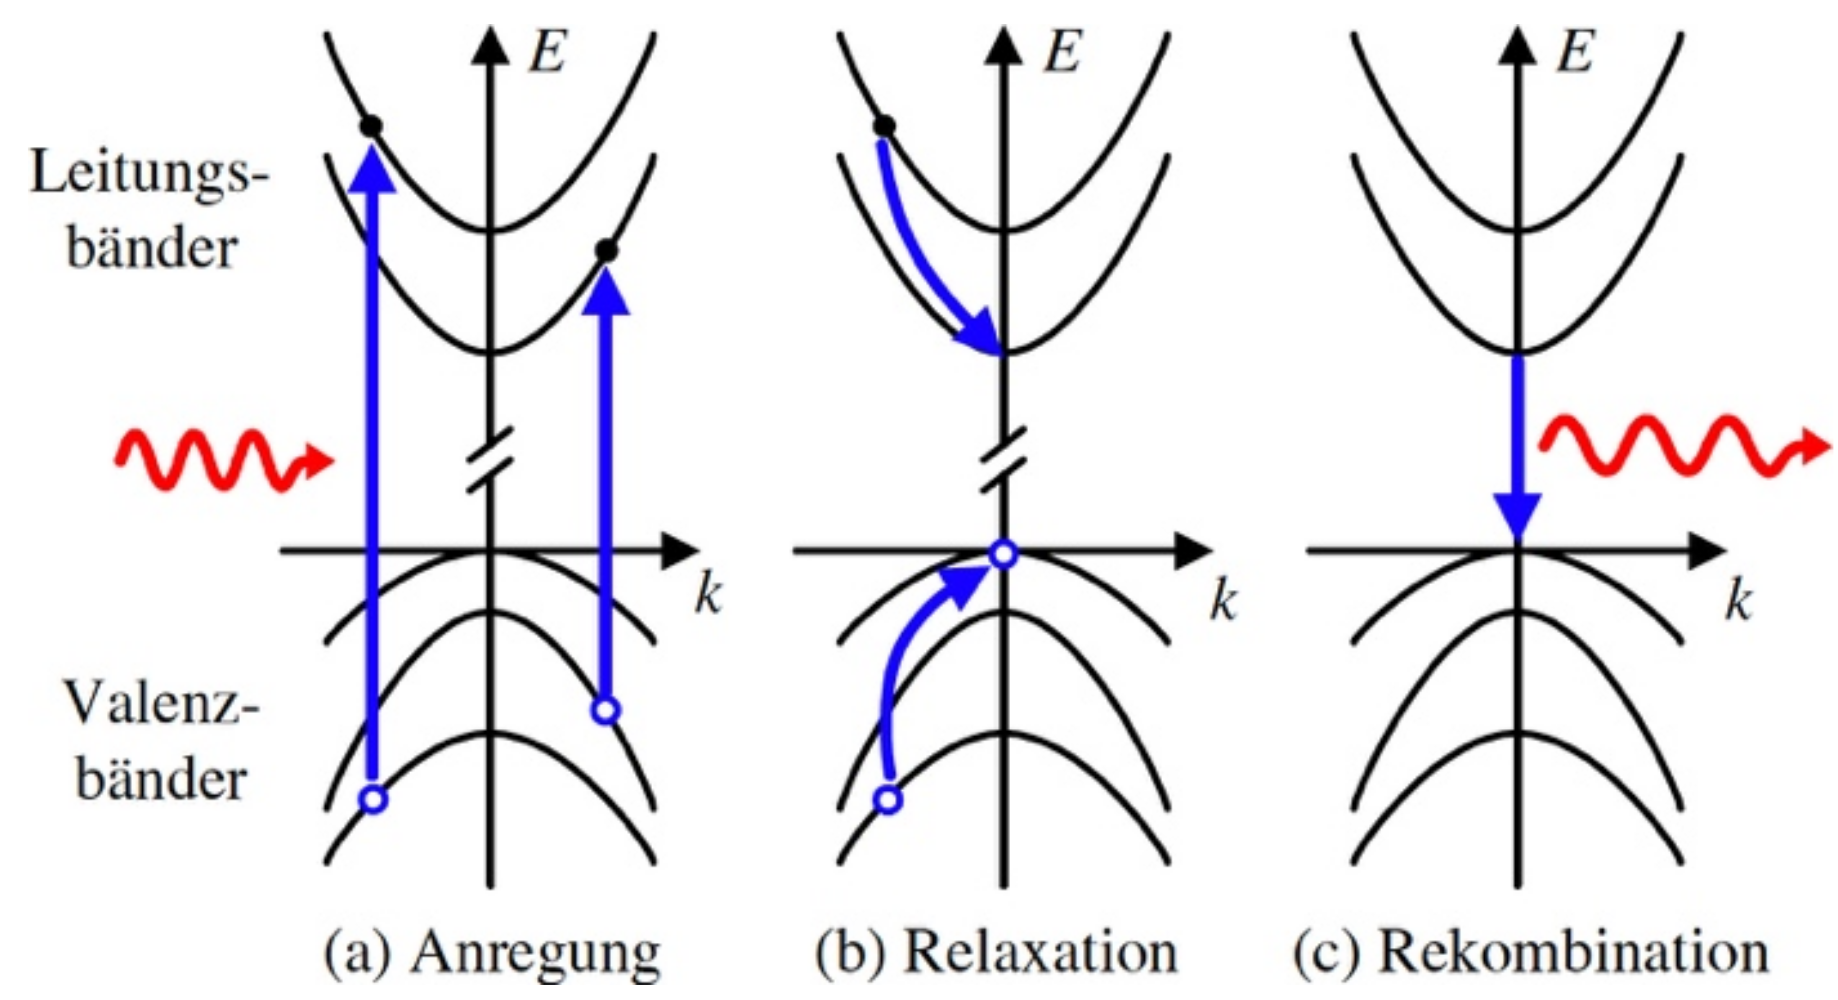
\includegraphics[width = 0.5\textwidth]{pics/PL.png}
  \caption{Prinzip der Photolumineszenz an Halbleitern anhand der drei Schritte Anregung, Relaxation und Rekombination \cite{anleitung_pl}.}
  \label{fig: pl}
\end{figure}


\subsection{Nanokristalle}
Zum Verständnis von Halbleiternanostrukturen ist eine Betrachtung von Banddiagrammen unverzichtbar\footnote{"\textit{If,
in discussing a semiconductor problem, you cannot draw an Energy-Band-Diagram, this shows
that you don't know what you are talking about. If you can draw one, but don't, then your audience
won't know what you are talking about.}"  - H. Krömer}. In solchen Diagrammen sind
die Unterseite des Leitungsbandes und die Oberkante des Valenzbandes einer Heterostruktur gegen eine
räumliche Achse aufgetragen.
\begin{figure}
  \centering
  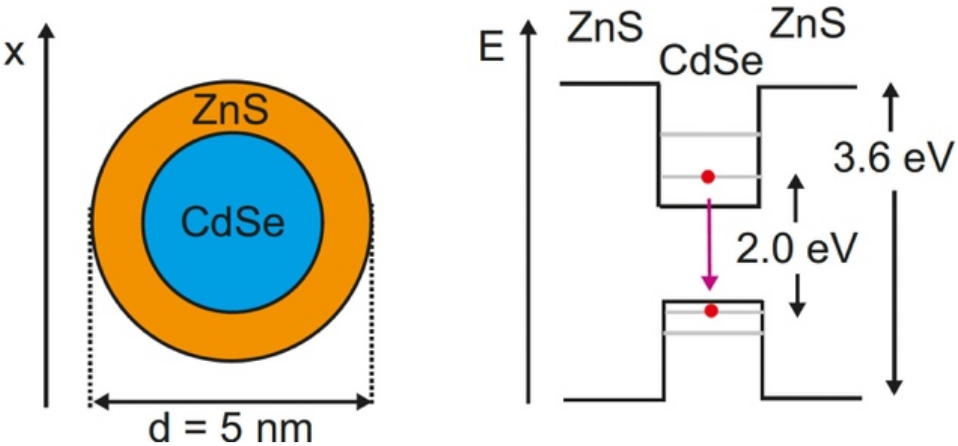
\includegraphics[width = 0.5\textwidth]{pics/banddiagramm.png}
  \caption{Schematische Darstellung eines Nanokristalls aus \ce{CdSe} und \ce{ZnS} (links) und
  das zugehörige Banddiagramm (rechts) \cite{anleitung_pl}.}
  \label{fig: energy_diagram}
\end{figure}
Abbildung~\ref{fig: energy_diagram} zeigt ein solches Diagramm für das hier untersuchte System aus \ce{CdSe} und
\ce{ZnS}. Die räumliche Achse verläuft durch den Mittelpunkt der kugelförmigen Struktur. Aufgrund der Tatsache, dass
die Bandlücke von \ce{CdSe} geringer ist als die von \ce{ZnS}, stellt der Verlauf der Bandkanten sowohl für Elektronen, als auch
für Löcher einen dreidimensionalen Potentialtopf im Inneren der Struktur dar. Die optische Anregung eines Elektron-Loch-Paares
kann nun direkt innerhalb des Topfes stattfinden, sobald die Energie die Bandlückenenergie von \ce{CdSe} übersteigt. Ist die
Anregungsenergie größer als die Bandlücke von \ce{ZnS}, so können auch hier Elektron-Loche-Paare erzeugt werden, die dann
anschließend im Quantentopf eingefangen werden.

Das Spektrum der Elektronen bzw. Löcher,
die sich innerhalb des Topfes befinden, lässt sich vereinfacht durch Lösung der Schrödingergleichung berechnen:
\begin{equation}
  \left[-\frac{\hbar^2}{2 m} \nabla^2 + V(\vec{r}) \right] \Psi(\vec{r}) = E \Psi(\vec{r}), \quad
  V(\vec{r}) = \begin{cases}
0,& \quad r > a\\
-V_0,& \quad r \leq a
\end{cases}
\end{equation}
mit der Ausdehnung des Quantentopfes $a$ und dem Einschlusspotential $V_0$.
Im Eindimensionalen Fall lassen sich die Energiezustände
anhand einer Quantenzahl $n \in N$ beschreiben:
\begin{equation}
  E_n = \frac{\pi^2\hbar^2n^2}{ 2 m a^2}.
  \label{eq: qw_energy}
\end{equation}
Es zeigt sich also, dass die Energien, die letztlich die Lumineszenzenergien festlegen, durch die Größe $a$ der Nanokristalle
moduliert werden können. Diese Eigenschaft bleibt auch im dreidimensionalen Fall erhalten, wobei hier zur Beschreibung der
Energieniveaus $E_{n, l}$ noch eine Drehimpulsquantenzahl $l \in N$ benötigt wird. Der Grundzustandsenergie
$(n = 1, l = 0)$ ist jedoch ebenfalls durch~\eqref{eq: qw_energy} mit $n = 1$ gegeben. Für die Energie $E_R$, die bei Rekombination eines
Elektrons mit einem Loch im Grundzustand frei wird, gilt daher
\begin{equation}
  E_R = E_g + \frac{\pi^2\hbar^2}{ 2  a^2} \left(\frac{1}{m_e^*} + \frac{1}{m_h^*}\right),
\end{equation}
mit den effektiven Massen von Elektron und Loch $m_e^*$ und $m_h^*$

Neben dem Potentialverlauf der Nanostruktur muss ebenfalls die Wechselwirkung zwischen Elektronen und Löchern berücksichtigt werden.
Diese lässt sich durch das Exziton-Modell beschreiben. Hierin werden Elektronen und Löcher wie freie Teilchen behandelt, die eine
Coulomb-Anziehung aufeinander ausüben. Die Wechselwirkung mit der Umgebnung wird duch eine relative Permeabilität
$\varepsilon_r$ moduliert. Es lassen sich so in Analogie zum Wasserstoffatom Bindungsenergien $E_m$ ($m \in N$) finden
\begin{equation}
  E_m = \frac{\mu e^4}{2 (4\pi\varepsilon_0 \varepsilon_r \hbar)^2} \cdot \frac{1}{m^2},
\end{equation}
mit der reduzierten Masse $\mu = \sfrac{m_e^* \cdot m_h^*}{(m_e^* + m_h^*)}$.
Hierdurch entstehen quantisierte Energiezustände innerhalb der
Bandlücke des Materials. Zusätzlich muss noch, anders als im Volumenhalbleiter, der Einfluss der räumlichen
Einschränkung der Elektronen und Löcher berücksichtigt werden. Hierdurch ergibt sich ein letzter Summand mit einer
$\sfrac{1}{a}$-Abhängigkeit \cite{}, der die Übergangsenergie beeinflusst. Es gilt damit insgesamt für die
Rekombinationsenergie im Grundzustand
\begin{equation}
  E_R = E_g + \frac{\pi^2\hbar^2}{ 2  a^2} \left(\frac{1}{m_e^*} + \frac{1}{m_h^*}\right) -\frac{\mu e^4}{2 (4\pi\varepsilon_0 \varepsilon_r \hbar)^2}
  - \num{1.786} \frac{e^2}{4\pi\varepsilon_r\varepsilon_0 a}.
  \label{eq: E_R}
\end{equation}
Dieses Modell kann verwendet werden, um aus gemessenen Photolumineszenzspektren den Durchmesser der Nanosphären $a$ zu bestimmen.

Die Intensität der Photolumineszenz wird wesentlich durch die Intensität der anregenden Laserstrahlung beeinflusst.
Dies geht damit einher, dass die Intensität der Photoluminszenz mit der Besetzungswahrscheinlichkeit der
Quantentrogzustände verknüpft ist. Diese Wahrscheinlichkeit steigt mit der anregenden Intensität (sprich mit der Zahl
an Photonen, die zur Anregung beitragen können).
Zudem steigt mit der anregenden Intensität auch die Wahrscheinlichkeit, Rekombinationen aus angeregten Zuständen
zu beobachten und mehr als ein Elektron-Loch-Paar
in einem Quantentrog anzutreffen.
Durch die gegenseitige Coulombwechselwirkung kann durch Letzteres auch die
Rekombinationsenergie aus dem Grundzustand \eqref{eq: E_R} verschoben werden. Grundsätzlich würde dies dazu führen, dass
mehrere Peaks im Spektrum zu erkennen sind. Da aber hier stets nur eine Mittlung über viele Nanokristalle vermessen wird,
kann höchstens eine Variation in der Breite der auftretenden Peaks als Indiz für eine veränderte Wahrscheinlichkeit der
Besetzung verschiedener Zustände beobachtet werden.
Insgesamt sind also Änderungen in der Intensität, spektralen Breite und spektralen Position der Photolumineszenz-Peaks
unter Variation der anregenden Leistung zu erwarten.
